%If you start a line with a "percent" symbol (like %), then that line is a "comment" and won't show up in your actual document.  

%Every document starts with a documentclass. 
\documentclass[11pt]{article}
\usepackage{titling}


%After that, it's useful to list an author and give a title.
\author{David Corneliu Turturean \& Daria Teodora Hărăbor}
\date{April 24, 2025} 
\title{%
  \textrm{Bayesian Inference of $\Lambda$CDM Model Parameters from CMB Temperature Anisotropies}\\[1ex]
  {\large\itshape Physics 212 Spring 2025}%
}
\author{David Corneliu Turturean \& Daria Teodora Hărăbor}
\date{April 24, 2025}
\raggedbottom

% 1) Load biblatex (so numeric style defines \labelnumbersep)
\usepackage[
  backend=biber,
  style=numeric,
  sorting=none
]{biblatex}
\addbibresource{myrefs.bib}

% 2) hyperref setup
\PassOptionsToPackage{colorlinks,linkcolor=blue,citecolor=blue,urlcolor=blue}{hyperref}
\usepackage{xcolor}
\usepackage{hyperref}
\usepackage{makecell}

% 3) Now override the bracketed labels and define the spacing
\DeclareFieldFormat{labelnumber}{#1}      % print “1.”
\renewcommand*{\bibopenbracket}{}          % drop “[”
\renewcommand*{\bibclosebracket}{}         % drop “]”
\setlength{\labelnumberwidth}{1.5em}       % width reserved for “1.”
%\setlength{\labelnumbersep}{0.5em}         % gap after “1.”


%The AMS packages. They contain a lot of useful math-related goodies.
\usepackage{amsthm}
\usepackage{amsmath}
\usepackage{amsfonts}
\usepackage[bottom]{footmisc}
\usepackage{hyperref}
\usepackage{booktabs}
\usepackage[most]{tcolorbox}
\usepackage{booktabs}
\usepackage{array}
\usepackage{booktabs}
\usepackage{xcolor}
\usepackage{tabularx}     % in your preamble


%This package changes the margins (makes them smaller than the default). 
\usepackage[margin=1in]{geometry}


%This package gives flexibility to use lettered lists in addition to numbered lists
\usepackage[shortlabels]{enumitem}

%The below command makes sure that every section starts on a new page. That way if you have a new section for every CA, they'll all print out on separate pieces of paper. 
\usepackage{titlesec}
\usepackage{amsmath}
\usepackage{amssymb}
%\newcommand{\sectionbreak}{\clearpage}

%The amsthm package lets you format different types of mathematical ideas nicely. You use it by defining "\newtheorem"s as below:
\newtheorem{problem}{Problem}
\newtheorem{theorem}{Theorem}
\newtheorem*{proposition}{Proposition}
\newtheorem{lemma}[theorem]{Lemma}
\newtheorem{corollary}[theorem]{Corollary}
\theoremstyle{definition}
\newtheorem{defn}[theorem]{Definition}
\renewcommand*{\proofname}{Solution} %This command changes "Proof" to "Solution" in the proof environment. 

%The "\newcommand" command lets you specify a custom command. This should be used wisely to add semantic meaning to otherwise confusing sequences of
%commands - not just speed up typing.
%Here is an example definition of a bra and ket from Quantum Mechanics.
\newcommand{\bra}[1]{\langle #1 |}
\newcommand{\ket}[1]{| #1 \rangle}
\newcommand{\erf}{\mathrm{erf}}    


%Adding your name here lets you make sure every page has your name, so that your psets don't get mixed up.
\usepackage{fancyhdr}
\pagestyle{fancy}
\lhead{David Corneliu Turturean \& Daria Teodora Hărăbor}
\rhead{Physics 212, Final Project}

%This changes removes indentation and instead adds space between paragraphs. I think it looks nicer this way. 
\setlength{\parindent}{0pt}
\setlength{\parskip}{1.25ex}


\begin{document}

\maketitle

\tableofcontents

\newpage

\section{Theory \& Background}
\label{sec:theory}

\subsection{$\Lambda$CDM Cosmological Model}

\subsubsection{Core Parameters}
In this project we use Bayesian inference to calculate the probability distributions of the six parameters of the \(\Lambda\)CDM model (Lambda Cold Dark Matter model),
\(\Theta=\{H_0,\Omega_b h^2,\Omega_c h^2,n_s,A_s,\tau\}\), from the Planck 2018 data \cite{planck2018params} on the CMB temperature using a Monte Carlo Markov Chain likelihood analysis (referred throughout this paper as MCMC) with the Metropolis Hastings algorithm. Below, we summarize the theory that connects the CMB temperature power spectrum to our parameters.

\begin{table}[h!]
  \centering
  \small
  \caption{$\Lambda$CDM parameters and their descriptions.}
  \label{tab:params_short}
  \begin{tabular}{c l}
    \toprule
    \multicolumn{1}{c}{\textbf{Parameter}} & 
    \multicolumn{1}{c}{\textbf{Description}} \\
    \midrule
    $H_0$           & Hubble constant, which determines the current expansion rate of the Universe [km\,s$^{-1}$\,Mpc$^{-1}$] \\
    $\Omega_bh^2$   & Physical baryon density                                                                             \\
    $\Omega_ch^2$   & Physical cold dark matter density                                                                   \\
    $n_s$           & Scalar spectral index, which describes the scale-dependence of primordial fluctuations               \\
    $A_s$           & Amplitude of the primordial scalar perturbations [$10^{-9}$]                                        \\
    $\tau$          & Optical depth to reionization                                                                       \\
    \bottomrule
  \end{tabular}
\end{table}


\subsubsection{Cosmological Dynamics}
In a flat universe, the Hubble parameter is a function of redshift \(z\):
\begin{equation}
  H(z)
  = H_0\,\sqrt{\Omega_m(1+z)^3 + \Omega_r(1+z)^4 + \Omega_\Lambda}\,,
  \qquad
  \Omega_m = \Omega_b + \Omega_c\,.
\end{equation}

Here, $H_0$ is the Hubble constant, $\Omega_m$ is the total matter density parameter (sum of baryon density parameter $\Omega_b$ and cold dark matter density parameter $\Omega_c$), $\Omega_r$ is the radiation density parameter, and $\Omega_\Lambda$ is the dark energy density parameter. At late cosmological times, \(\Omega_r\) is negligible. We also define
\( h \) such that 
\(H_0 = 100\,h\ \mathrm{km\,s^{-1}Mpc^{-1}}\), where $h$ is the dimensionless Hubble parameter.

\subsubsection{Sound Horizon and Acoustic Scale}
The comoving sound horizon at photon decoupling redshift (\(z_*\)) sets the characteristic scale
of the acoustic peaks of the power spectrum:
\begin{equation}
  r_s(z_*) 
  = \int_{z_*}^\infty \frac{c_s(z)}{H(z)}\,dz,
  \quad
  c_s(z) = \frac{c}{\sqrt{3\bigl[1+R(z)\bigr]}},
  \quad
  R(z)=\frac{3\rho_b(z)}{4\rho_\gamma(z)}.
\end{equation}

In these equations, $c_s(z)$ is the sound speed in the baryon-photon fluid, $c$ is the speed of light, $R(z)$ is the ratio of baryon to photon density, $\rho_b(z)$ is the baryon density, and $\rho_\gamma(z)$ is the photon density.

\subsubsection{Density Parameters and Critical Density}
The actual densities relate to the aforementioned density parameters as follows:
\begin{equation}
   \rho_i(z) = \rho_{\mathrm{crit},0} \, \Omega_i \, (1+z)^{3(1+w_i)},
  \qquad
  \rho_{\mathrm{crit},0} = 3H_0^2/(8\pi G),
\end{equation}

  Here, \( \rho_{\mathrm{crit},0} \) is the critical density
  today, and \( w_i \) is the equation of state parameter for component \( i \in \{ m, r, \Lambda \}\): \( w \) is 0 for matter, 1/3 for radiation, and -1 for dark energy.   
  
  We can thus see that the density
  parameters $\Omega_i$ are defined as the ratio of the current energy density (when \( z = 0\)) to the critical density: $\Omega_i =
  \rho_{i,0}/\rho_{\mathrm{crit},0}$.

The comoving angular diameter distance to the last scattering surface is:
\begin{equation}
  D_A(z_*) 
  = \frac{1}{1+z_*}\int_0^{z_*}\frac{c\,dz}{H(z)}.
\end{equation}

Furthermore, a key feature in the CMB power spectrum is the series of acoustic peaks, which result from sound waves in the photon-baryon plasma before recombination \cite{hu2002}. The acoustic scale $\ell_A$ predicts the location of the first peak in multipole space and is given by:
\begin{equation}
  \ell_A = \pi\,\frac{D_A(z_*)}{r_s(z_*)}\,,
\end{equation}
Based off previous observations, we expect the peak to be at $l\approx 220$.

\subsubsection{Wavenumber-Multipole Relation}
Each multipole $\ell$ corresponds to a wavenumber, approximately as such:

\begin{equation}
k \approx \frac{\ell}{r(z_*)}
\end{equation}

\subsubsection{Primordial Power Spectrum}
We use the wavenumbers to parametrize the primordial curvature power spectrum $P_{\mathcal{R}}(k)$ as:
\begin{equation}
  P_{\mathcal R}(k)
  = A_s\bigl(\tfrac{k}{k_0}\bigr)^{n_s-1},
\end{equation}

where $A_s$ is the amplitude of scalar perturbations, $n_s$ is the scalar spectral index, and \(k_0\) is the pivot scale where we measure $n_s$ (typically $k_0 = 0.05$ Mpc$^{-1}$).


\subsubsection{Angular Power Spectrum}
A Boltzmann solver (such as CAMB, the Code for Anisotropies in the Microwave Background) can evolve 
\(P_{\mathcal R}(k)\)
through recombination to yield the theoretical angular power spectrum, for which we employ:
\begin{equation}
  C_\ell^{\rm th}
  = \frac{1}{2\ell+1}\sum_{m=-\ell}^{\ell}\bigl|a_{\ell m}^{\rm th}\bigr|^2.
\end{equation}

Here, $a_{\ell m}^{\rm th}$ are the coefficients in the spherical harmonic decomposition of the predicted CMB temperature field.

We use an analogous formula to obtain the observed angular power spectrum, using the coefficient in the spherical harmonic composition of the measured CMB temperature field:

\begin{equation}
  C_\ell^{\rm obs}
  = \frac{1}{2\ell+1}\sum_{m=-\ell}^{\ell}\bigl|a_{\ell m}^{\rm obs}\bigr|^2.
\end{equation}

\subsubsection{Physical Effects on the Power Spectrum}
We modify the theoretical power spectrum to account for two important physical effects:

\begin{align}
  &C_\ell^{\rm th} \to C_\ell^{\rm th}  \exp\bigl(-\ell^2/\ell_D^2\bigr)
  \text{where }\ell_D\text{ is the diffusion (Silk damping) scale},\\
  &C_\ell^{\rm th}\to C_\ell^{\rm th}\,e^{-2\tau},
  \quad
  \text{where }\tau\text{ is the optical depth to reionization}.
\end{align}

The first effect, Silk damping, suppresses power at small scales due to photon diffusion \cite{silk1968}, while the second effect accounts for the rescattering of CMB photons during the epoch of reionization.

\subsubsection{Diffusion (Silk Damping) Scale}
The Silk damping scale $\ell_D$ characterizes the exponential suppression of power at small scales due to photon diffusion. We calculate it as:
\begin{equation}
\ell_D = k_D d_A(z_*),
\end{equation}

  where $k_D$ is the physical damping wavenumber. The damping wavenumber can be calculated directly from the fundamental physics of photon diffusion in the early universe:

\begin{equation}
k_D^{-2} = \frac{1}{6} \int_{0}^{z_*} \frac{dz}{H(z)} \frac{1+z}{\sigma_T n_e(z) a} \frac{{R(z)}^2 + \frac{16}{15}(1+R(z))}{(1+R(z))^2},
\end{equation}

where $\sigma_T$ is the Thomson cross-section (physical constant), and $n_e(z)$ is the free electron number density, which depends on the baryon density: $n_e(z) \propto \Omega_b h^2 (1+z)^3$.

The integral can be evaluated numerically using our six $\Lambda$CDM parameters without relying on previously calibrated coefficients. The result depends most strongly on $\Omega_b h^2$ and $\Omega_m h^2$.

For computational efficiency in our MCMC implementation, we approximate this calculation with a scaling relation that captures the essential parameter dependencies, as motivated in Appendix~\ref{sec:appendix_silk}:

\begin{equation}
\ell_D \approx k_D d_A(z_*) \approx 1600 \left(\frac{\Omega_b h^2}{0.02237}\right)^{-0.25} \left(\frac{\Omega_m h^2}{0.1424}\right)^{-0.125}
\end{equation}


\subsection{Illustrative Semi‑Analytic TT Spectrum Model}
\textit{Note: This section presents a simplified model for conceptual understanding only. Our actual parameter inference uses the full Boltzmann solver calculations described in Section 1.1.}

For pedagogical purposes, we can illustrate the key features of the CMB power spectrum using a simplified semi-analytic model, putting together the aforementioned formulas in approximate fashion. This visual representation captures the essential physics. We define the CMB power spectrum in terms of $D_{\ell}$, which is a rescaled version of the angular power spectrum $C_{\ell}$:
\[
D_\ell \equiv \frac{\ell(\ell+1)}{2\pi}\,C_\ell
\]


\[
D_\ell \approx A_s \,\Bigl(\tfrac{k}{k_0}\Bigr)^{n_s-1}
\;\sin^2\!\bigl(\tfrac{\pi\ell}{\ell_{\rm ac}}\bigr)
\;\exp\!\Bigl[-\bigl(\tfrac{\ell}{\ell_D}\bigr)^2\Bigr]
\;e^{-2\tau}\times10^{9}\,,
\]
where:
\begin{itemize}
  \item $P(k)=A_s\,(k/k_0)^{n_s-1}$ is the primordial power spectrum (pivot scale $k_0=0.05\,\mathrm{Mpc}^{-1}$),
  \item $\sin^2(\pi\ell/\ell_{\rm ac})$ approximates the acoustic oscillations,
  \item $\exp[-(\ell/\ell_D)^2]$ is a Gaussian Silk‑damping envelope,
  \item $e^{-2\tau}$ applies the reionization suppression,
  \item the factor $10^9$ converts the power spectrum to $\mu{\rm K}^2$ units (microkelvin squared).
\end{itemize}

This simplified formula provides the intuition behind the more complex calculations used in our actual parameter inference pipeline.


\begin{figure}[htbp]
  \centering
  \includegraphics[scale=1]{semianalytic.png}
  \caption{Comparison of semi‑analytic CMB TT power spectrum with Planck 2018 data [\cite{planck2018}].}
  \label{fig:cmb-tt-comparison}
\end{figure}

\section{Methods}

\subsection{Likelihood Function}

To constrain cosmological parameters, we need to compare our theoretical model with the observed data. The exact likelihood for each multipole $\ell$ is given by the $\chi^2$ distribution:

\begin{equation}
  \mathcal{L}_\ell \propto \frac{(2\ell+1)}{2C_\ell^{\rm th}} 
  \left(\frac{C_\ell^{\rm obs}}{C_\ell^{\rm th}}\right)^{\frac{2\ell-1}{2}} 
  \exp\left[-\frac{(2\ell+1)C_\ell^{\rm obs}}{2C_\ell^{\rm th}}\right],
\end{equation}

This exact form reflects the fact that for each multipole $\ell$, we have $2\ell+1$ independent modes (corresponding to $m$ values from $-\ell$ to $\ell$), and the power spectrum estimator follows a $\chi^2$ distribution with $2\ell+1$ degrees of freedom. 

For high multipoles ($\ell \gtrsim 30$), the number of modes becomes large, and by the central limit theorem, the log-likelihood summed over multipoles can be written as the following \cite{bond2000} (see Appendix~\ref{app:gaussian} for mathematical details):

\begin{equation}
  -2\ln\mathcal{L}(\Theta)
  \approx \sum_{\ell=\ell_{\min}}^{\ell_{\max}}
    \frac{\bigl[C_\ell^{\rm th}(\Theta)-C_\ell^{\rm obs}\bigr]^2}
         {\sigma_\ell^2},
  \quad
\end{equation}
\begin{equation}
  \sigma_\ell = \sqrt{\frac{2}{2\ell+1}}\,C_\ell^{\rm th}.
\end{equation}

Here, $\mathcal{L}(\Theta)$ is the likelihood function, $C_\ell^{\rm th}(\Theta)$ is the theoretical power spectrum corresponding to the $\Theta$ set of parameters, $C_\ell^{\rm obs}$ is the observed power spectrum, and $\sigma_\ell$ is the uncertainty in the power spectrum estimate derived from cosmic variance \cite{knox1995}. The sum runs from $\ell_{\min}$ to $\ell_{\max}$, which define the multipole range of our analysis. In our approach, we used $\ell_{\min}=30$ and $\ell_{\max}=2500$ for this Gaussian approximation. The variance $\sigma_\ell^2$ decreases with increasing $\ell$ due to the larger number of available modes.

For lower multipoles ($\ell<30$), where cosmic variance dominates and the number of modes is small, the Gaussian approximation breaks down. Here, one should either use the exact $\chi^2$ likelihood given in the first equation or adopt a hybrid approach where the exact form is used for low $\ell$ and the Gaussian approximation for high $\ell$.

\subsection{Markov Chain Monte Carlo with Temperature Annealing}

We sample the posterior distribution $P(\Theta\mid\mathrm{data})\propto \mathcal{L}(\Theta)\,\pi(\Theta)$ using a modified Metropolis--Hastings algorithm with temperature annealing \cite{lewis2002}. This approach helps navigate complex posterior landscapes with multiple local maxima and improves mixing of the chains.

\subsubsection{The Metropolis--Hastings Algorithm}

The standard Metropolis--Hastings algorithm generates a Markov chain that converges to the target posterior distribution. At each step $i$, starting from a current state $\Theta_i$, we:

\begin{enumerate}
\item Generate a proposal $\Theta'$ from a symmetric proposal distribution
\item Accept this proposal with probability
\begin{equation}
  \alpha = \min \left\{1,\,
    \frac{P(\Theta'\mid\mathrm{data})}{P(\Theta\mid\mathrm{data})}
  \right\} = \min \left\{1,\,
    \frac{\mathcal{L}(\Theta')\,\pi(\Theta')}
         {\mathcal{L}(\Theta)\,\pi(\Theta)}
  \right\}
\end{equation}
\item Update the chain according to
\begin{equation}
  \Theta_{i+1} =
  \begin{cases}
    \Theta' & \text{if }u<\alpha,\\
    \Theta_i & \text{otherwise},
  \end{cases}
  \quad u\sim\mathcal{U}(0,1)
\end{equation}
\end{enumerate}

\subsubsection{Temperature Annealing Extension}

To enhance exploration of the parameter space, we implement temperature annealing. This technique borrows from statistical physics and defines a ``temperature'' parameter $T$ that initially flattens the posterior landscape, then gradually restores it to its true shape.

At iteration $n$ of a total $N$ iterations, we modify the standard acceptance probability by introducing a temperature-dependent distribution:

\begin{equation}
P_{T_n}(\Theta\mid\mathrm{data}) \propto [P(\Theta\mid\mathrm{data})]^{1/T_n}
\end{equation}

This results in a modified acceptance probability:

\begin{equation}
\alpha = \min \left\{1,\,
\left[\frac{P(\Theta'\mid\mathrm{data})}{P(\Theta\mid\mathrm{data})}\right]^{1/T_n}
\right\} = \min \left\{1,\,
\left[\frac{\mathcal{L}(\Theta')\,\pi(\Theta')}{\mathcal{L}(\Theta)\,\pi(\Theta)}\right]^{1/T_n}
\right\}
\end{equation}

The temperature decreases according to an exponential cooling schedule: 
\begin{equation}
T_n = T_0\left(\frac{T_f}{T_0}\right)^{n/N}
= T_0\exp\left(-\frac{n}{N}\ln\frac{T_0}{T_f}\right),
\end{equation}

with initial temperature $T_0=5$ (hot, flat landscape) and final temperature $T_f=1$ (true posterior). Early in the chain ($n\approx0$), the high temperature makes it easier to traverse the parameter space; later ($n\to N$), $T_n\to1$ ensures we sample from the exact posterior distribution.

When $T_n > 1$, the posterior becomes flatter, making it easier for the chain to traverse valleys. At the end of the annealing schedule ($T_n = 1$), we recover the standard Metropolis--Hastings algorithm.

\subsubsection{Assessing Convergence}

To assess convergence across multiple chains, we use the Gelman--Rubin statistic $\widehat{R}$. This diagnostic compares the between-chain variance to the within-chain variance for each parameter. When all chains have converged to the same stationary distribution, these variances should be approximately equal, giving $\widehat{R} \approx 1$. 

Formally, for each parameter $\theta_j$, if we have $m$ chains each of length $n$, we compute:
\begin{equation}
\widehat{R} = \sqrt{\frac{V}{W}}, \quad \text{where} \quad V = \frac{n-1}{n}W + \frac{1}{n}B
\end{equation}

Here $B$ is the between-chain variance and $W$ is the within-chain variance. Values $\widehat{R}\lesssim1.1$ are typically considered to indicate good mixing and convergence of the chains.







\subsection{Prior Choices for \(\Lambda\)CDM Parameters}

We adopt the following priors to incorporate prior knowledge about the parameters and to make sure we get robust inference results:

\begin{table}[htbp]
  \centering
  \small
  
  \label{tab:params_priors_expl}
  \begin{tabularx}{\textwidth}{@{} c c X @{}}
    \toprule
    \multicolumn{1}{c}{\textbf{Parameter}} & 
    \multicolumn{1}{c}{\textbf{Prior}} & 
    \multicolumn{1}{c}{\textbf{Reason for choosing prior}} \\
    \midrule

    $H_0$           & Uniform (50,\,90)                  & Reflects broad Hubble‐constant measurements (distance ladder, time‐delay lenses) without over‐constraining. \\[0.5ex]
    $\Omega_b h^2$  & Gaussian $\mathcal{N}(0.02237,0.0005^2)$ & Encodes precise BBN constraints from D/H and $^4$He abundances, independent of CMB TT data. \\[0.5ex]
    $\Omega_c h^2$  & Uniform (0.05,\,0.25)              & A wide non‐informative range accommodating both Planck and large‐scale‐structure estimates. \\[0.5ex]
    $n_s$           & Uniform (0.85,\,1.05)              & Covers inflationary predictions ($n_s\approx1$) while allowing mild deviations. \\[0.5ex]
    $A_s$           & Uniform (1,\,4)$\times10^{-9}$     & Flat over the plausible amplitude range inferred from CMB and large‐scale structure. \\[0.5ex]
    $\tau$          & Gaussian $\mathcal{N}(0.0544,0.0073^2)$ & Based on low‐$\ell$ polarization measurements (Planck 2018), with well‐characterized errors. \\
    \bottomrule
  \end{tabularx}
  \caption{$\Lambda$CDM parameters and chosen priors}
\end{table}

\newpage





\subsection{GitHub directory}
% in your preamble:

Now let us go through the \href{https://github.com/davidturturean/Phys212_Spring2025Project}{GitHub directory} and break down each of our files:

\newtcbox{\filebox}{%
  on line,
  colback=blue!10,      % box fill color
  arc=3pt,              % corner roundness
  boxrule=0pt,          % no border line
  boxsep=1pt,           % inner padding
  left=3pt,right=3pt,top=1pt,bottom=1pt
}
\newcolumntype{L}[1]{>{\raggedright\arraybackslash}p{#1}}  % for wrapping

\renewcommand{\arraystretch}{1.5} % Increase row spacing
\begin{table}[h!]
  \small

  \label{tab:codefiles_updated}
  \begin{tabular}{L{4.5cm} L{10.5cm}}
    \toprule
    \textbf{File} & \textbf{Description} \\
    \midrule
    \filebox{CAMB.py}                    & Power spectrum calculation using CAMB. \\
    \filebox{cosmology\_model.py}       & Implementation of $\Lambda$CDM cosmological model. \\
    \filebox{data\_loader.py}           & Functions to load Planck CMB data. \\
    \filebox{likelihood.py}            & Likelihood function for parameter estimation. \\
    \filebox{mcmc\_run.py}              & Standard MCMC implementation. \\
    \filebox{modified\_mcmc.py}         & Enhanced MCMC with temperature annealing. \\
    \filebox{parameters.py}            & Cosmological parameter definitions and priors. \\
    \filebox{priors.py}                & Prior distribution implementations. \\
    \filebox{theoretical\_lcdm.py}      & Theoretical predictions for $\Lambda$CDM. \\
    \filebox{analyze\_annealing\_chains.py}   & Analysis of temperature annealing chains. \\
    \filebox{analyze\_final\_steps.py}       & Analysis of final steps in annealing chains. \\
    \filebox{analyze\_standard\_chains.py}   & Analysis of standard MCMC chains. \\
    \filebox{compare\_annealing\_runs.py}    & Comparison between different annealing runs. \\
    \filebox{visualize\_constraints.py}      & Visualization of parameter constraints. \\
    \filebox{visualize\_model\_fits.py}      & Visualization of model fits to data. \\
    \filebox{compare\_with\_planck.py}       & Comparison with Planck 2018 results. \\
    \bottomrule
  \end{tabular}
  \caption{Code files used for $\Lambda$CDM parameter inference and analysis}
\end{table}


\bigskip

\section{Results \& Discussion}

\subsection{Parameter Estimates}

We present the results of $\Lambda$CDM cosmological parameter inference using two different MCMC methods: a standard sampler and a temperature annealing sampler. The inferred values and $68\%$ credible intervals for the cosmological parameters are summarized in Table $4$. Both methods yield broadly consistent results for most parameters, with notable deviations for $\Omega_c h^2$ and $n_s$. We note that for most parameters, the standard MCMC was statistically consistent with the Planck 2018 values ($<1\sigma$), whereas the annealing MCMC has two parameters with more significant deviations ($>2\sigma$).


\begin{figure}[htbp]
  \centering
  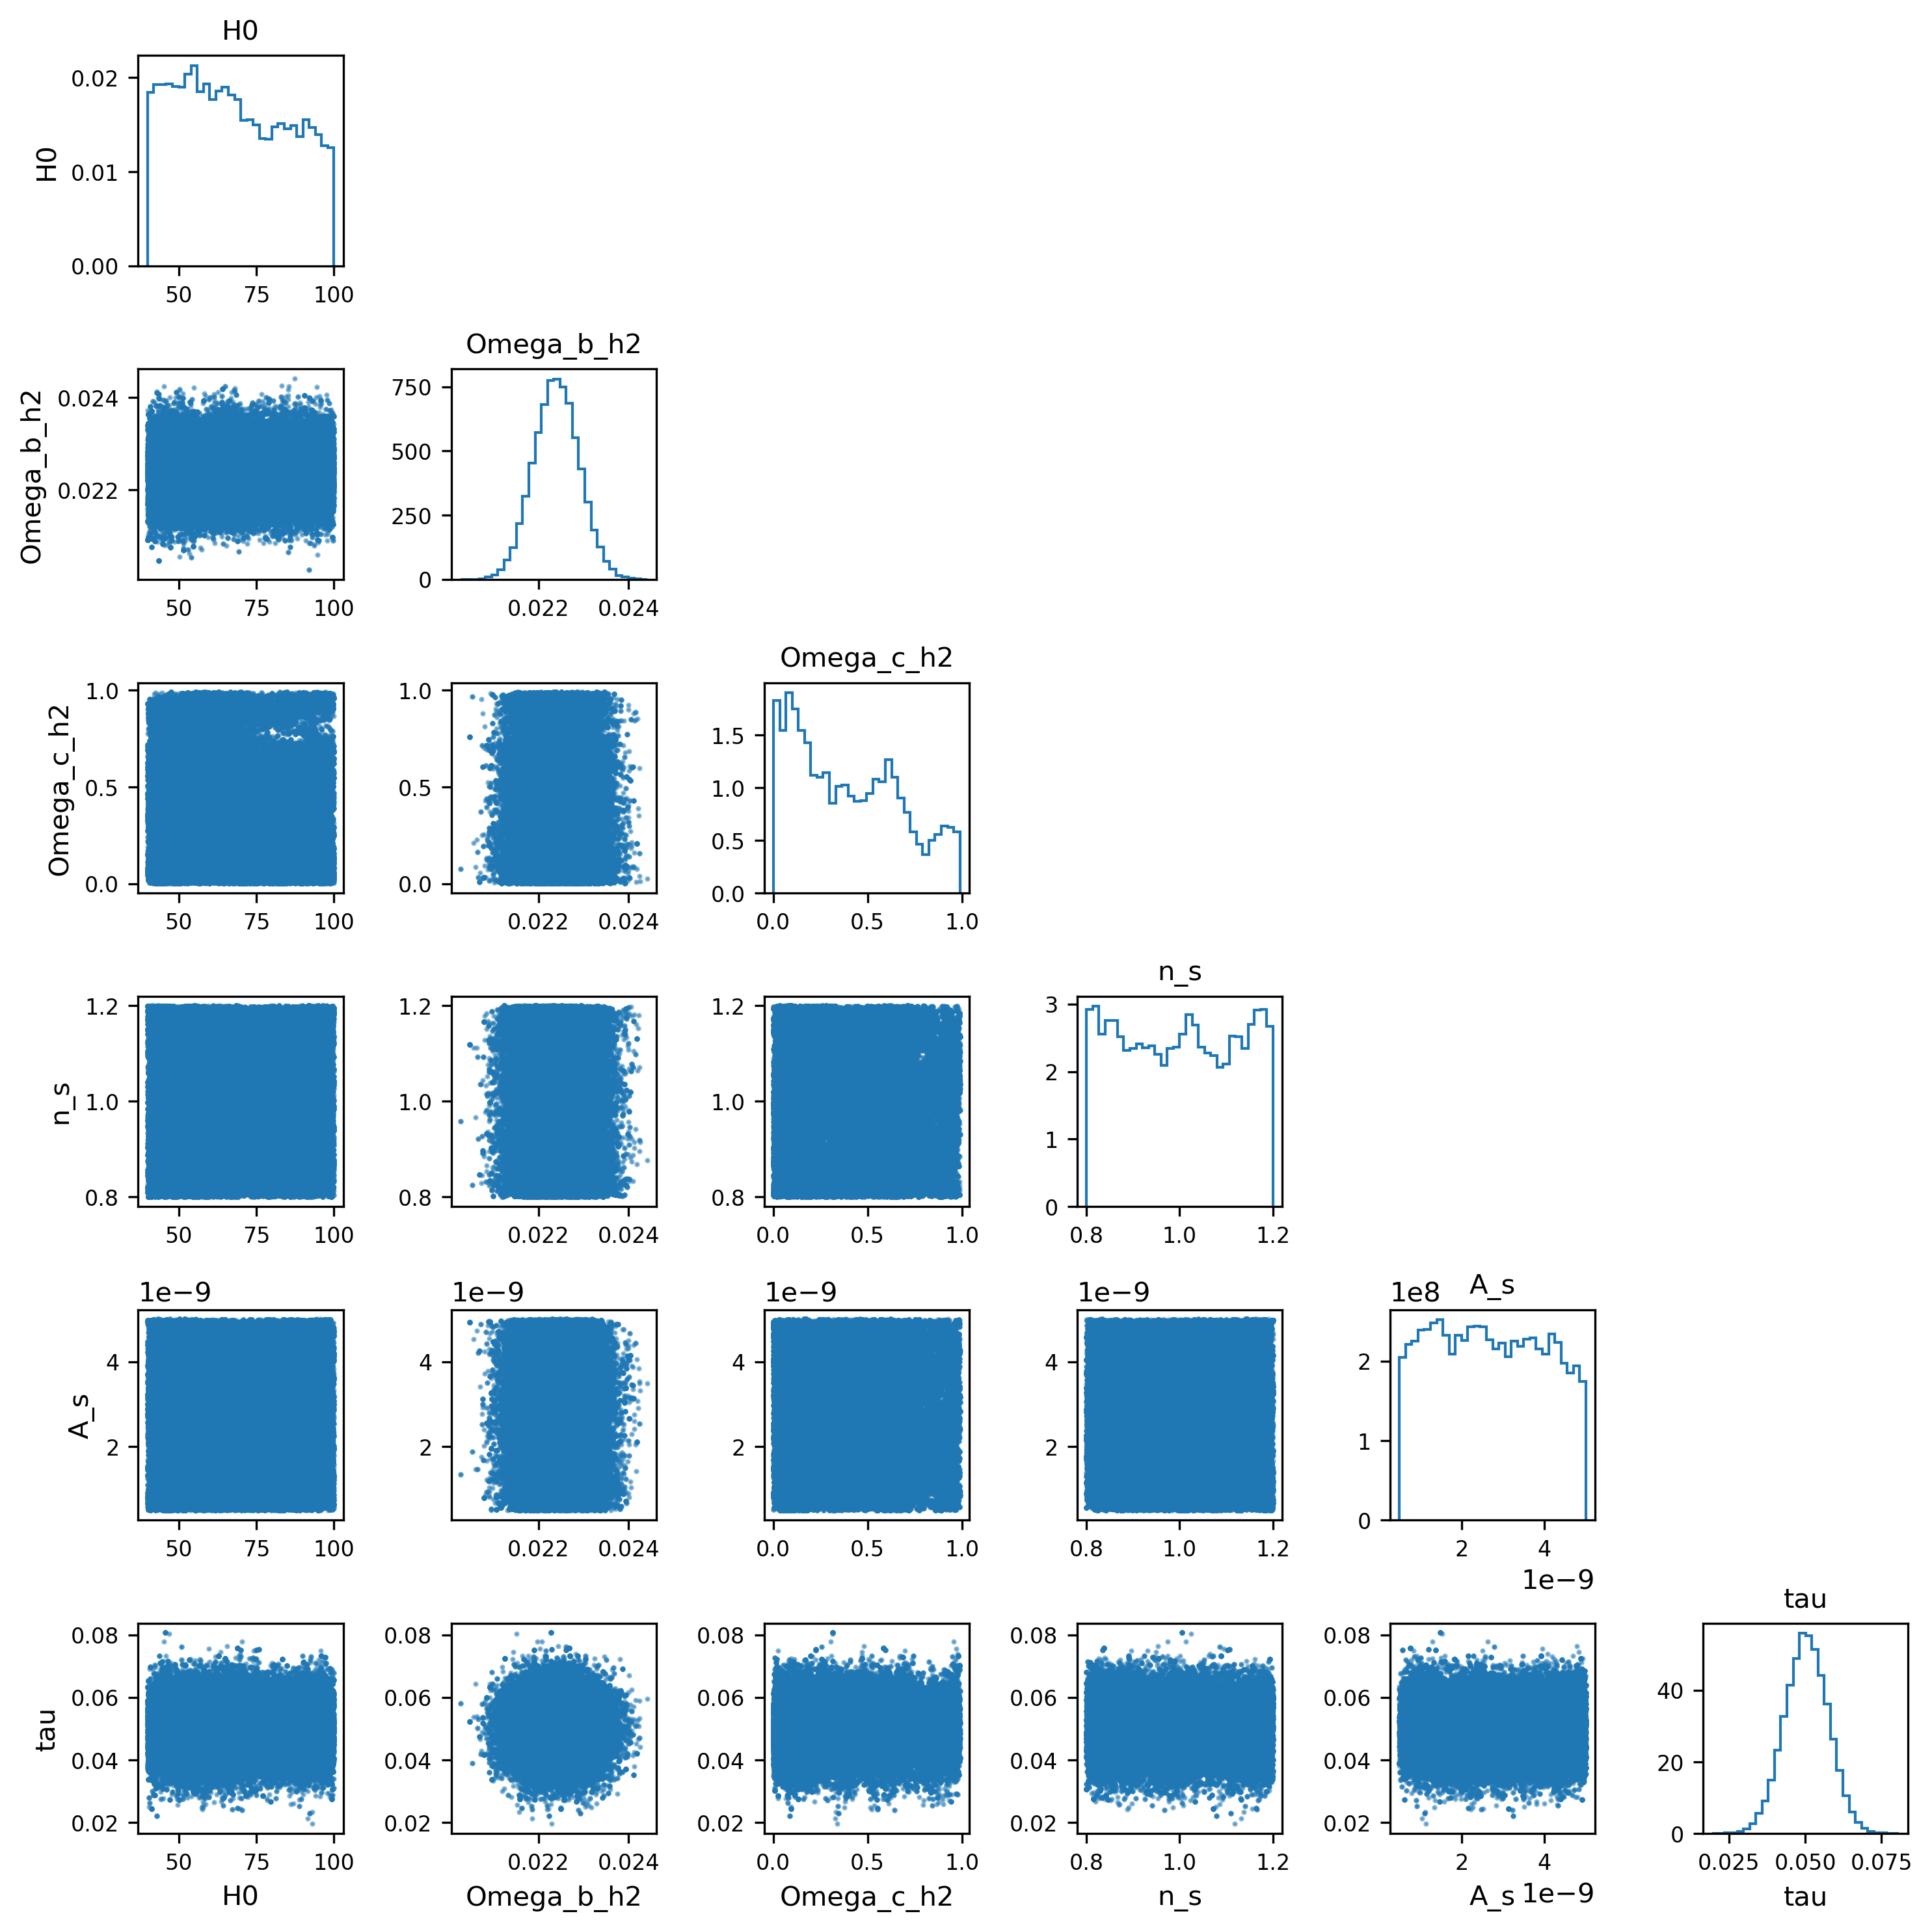
\includegraphics[scale=0.65]{standard_corner_plot.png}
  \caption{Corner plot of the standard MCMC analysis.}
  \label{fig:cmb-tt-comparison}
\end{figure}


\begin{figure}[htbp]
  \centering
  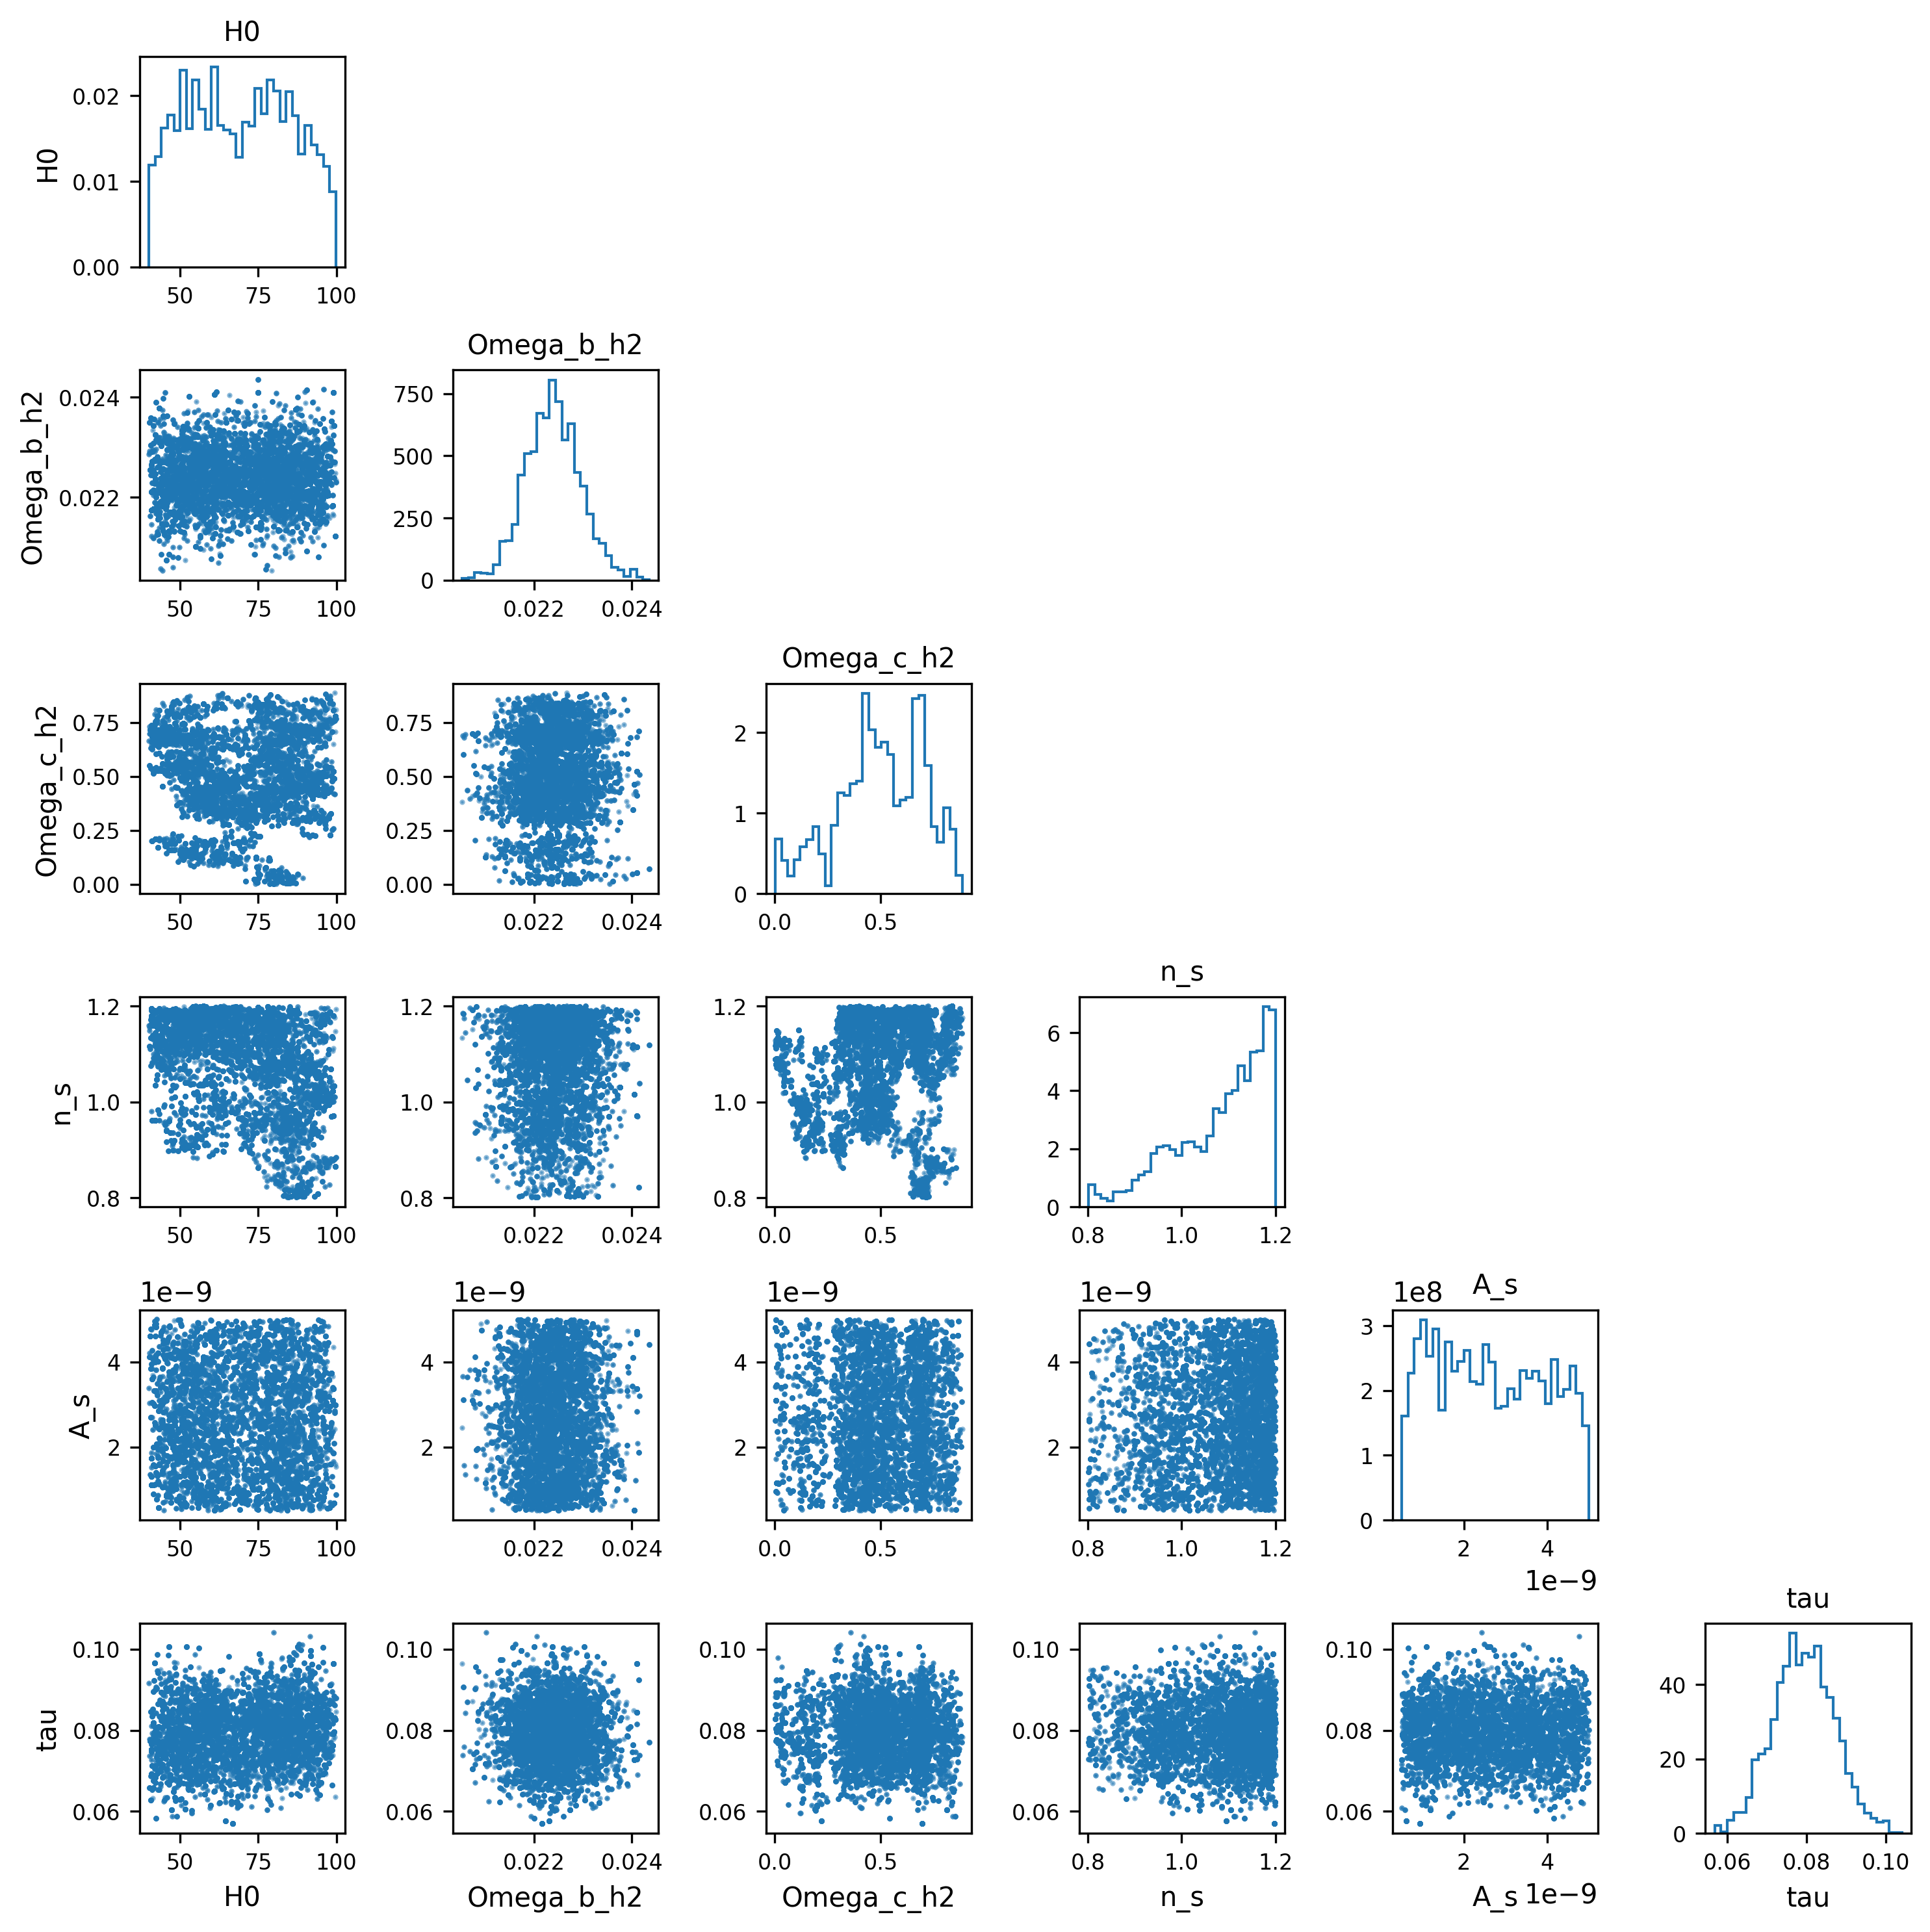
\includegraphics[scale=0.65]{annealing_corner_plot.png}
  \caption{Corner plot of the annealing MCMC analysis.}
  \label{fig:cmb-tt-comparison}
\end{figure}


\renewcommand{\arraystretch}{1.4}
\setlength{\tabcolsep}{3pt} % tighter spacing
\renewcommand{\arraystretch}{1.8} % More spacious
\begin{table}[h]
\centering

\label{tab:final_comparison_clean}
\begin{tabular}{c c c c c c}
\toprule
\textbf{Parameter} &
\textbf{Planck 2018} &
\textbf{Standard MCMC} &
\textbf{Annealing MCMC} &
\makecell{\textbf{Standard}\\\textbf{vs.}\\\textbf{Planck}} &
\makecell{\textbf{Annealing}\\\textbf{vs.}\\\textbf{Planck}} \\
\midrule
$H_0$ &
$67.4 \pm 0.5$ &
$66.11^{+22.41}_{-17.68}$ &
$69.56^{+19.16}_{-18.74}$ &
$0.06\sigma$ & $0.11\sigma$ \\
$\Omega_b h^2$ &
$0.0224 \pm 0.0001$ &
$0.022397^{+0.000502}_{-0.000503}$ &
$0.022374^{+0.000593}_{-0.000553}$ &
$0.01\sigma$ & $0.04\sigma$ \\
$\Omega_c h^2$ &
$0.120 \pm 0.001$ &
$0.3624^{+0.3401}_{-0.2696}$ &
$0.5135^{+0.1940}_{-0.1828}$ &
$0.71\sigma$ & $2.03\sigma$ \\
$n_s$ &
$0.965 \pm 0.004$ &
$1.0012^{+0.1411}_{-0.1441}$ &
$1.1056^{+0.0725}_{-0.1499}$ &
$0.25\sigma$ & $1.44\sigma$ \\
$A_s\times10^{-9}$ &
$2.10 \pm 0.03$ &
$2.645 \pm 1.544$ &
$2.524 \pm 1.529$ &
$0.35\sigma$ & $0.28\sigma$ \\
$\tau$ &
$0.054 \pm 0.007$ &
$0.0504^{+0.0071}_{-0.0071}$ &
$0.0792^{+0.0077}_{-0.0077}$ &
$0.25\sigma$ & $2.47\sigma$ \\
\bottomrule
\end{tabular}
\caption{Comparison of base $\Lambda$CDM parameters from Planck 2018, standard MCMC, and temperature annealing MCMC. Last columns show deviation significance from Planck 2018.}
\end{table}


\bigskip

\subsection{Convergence and Sampling Efficiency}

Standard MCMC suffered from convergence issues in several parameters. Gelman-Rubin $R\hat{}$ values exceeded the acceptable threshold ($R\hat{} > 1.1$) for four out of six parameters, most severely for $\tau$ ($R\hat{} = 2.17$). In contrast, the temperature annealing chains demonstrated significantly improved convergence, aided by a cooling schedule that enabled better exploration of the parameter space and avoidance of local likelihood maxima.

\renewcommand{\arraystretch}{1.2} % Reduce row height
\begin{table}[h]
\centering

\label{tab:rhat_comparison}
\begin{tabular}{lccc}
\toprule
\textbf{Parameter} & \textbf{Standard MCMC} & \textbf{Annealing MCMC} & \textbf{Converged?} \\
\midrule
$H_0$            & 1.0031 & 1.0032 & Yes/Yes \\
$\Omega_b h^2$   & 1.0002 & 1.0000 & Yes/Yes \\
$\Omega_c h^2$   & 1.2023 & 1.0031 & No/Yes \\
$n_s$            & 1.0411 & 1.0022 & Yes/Yes \\
$A_s$            & 1.0030 & 1.0000 & Yes/Yes \\
$\tau$           & 1.0002 & 1.0002 & Yes/Yes \\
\bottomrule
\end{tabular}
\caption{Gelman–Rubin $R\hat{}$ statistics for each parameter, comparing standard and temperature annealing MCMC chains. Convergence is assumed if $R\hat{} < 1.1$.}
\end{table}





\subsection{Credible Interval Comparison}

Temperature annealing produced tighter credible intervals for $H_0$, $\Omega_c h^2$, and $n_s$, reflecting a more efficient sampling of these dimensions. Notably, the width of the $68\%$ interval for $\Omega_c h^2$ decreased by $56.1\%$ and for $n_s$ by $34.7\%$. However, $\Omega_b h^2$ and $\tau$ showed slightly wider intervals under annealing, potentially due to more complete exploration of long-tailed or degenerate posteriors.

\subsection{Methodological Implications}

The annealing-based approach demonstrates clear advantages for high-dimensional or multimodal posterior surfaces, typical in cosmological inference. It enhances mixing, reduces sensitivity to initialization, and offers faster effective convergence. For future analyses, especially when tighter constraints are critical, we recommend using temperature annealing as the default sampling strategy, while maintaining standard MCMC as a validation tool.

\subsection{MCMC Implementation Details}

Our parameter inference utilized two complementary MCMC methodologies with distinct performance characteristics. Both implementations used a single-walker approach per chain rather than an ensemble sampler.

\subsubsection{Standard MCMC Configuration}

The standard MCMC implementation consisted of 4 chains, each running for 30,000 steps. After discarding the first 20\% as burn-in, we analyzed a total of 96,000 posterior samples (24,000 effective steps per chain). These chains were executed on the MIT Engaging cluster, requiring approximately 8-12 hours with an allocation of 16 CPUs and 64GB memory.

Proposal scales were fixed at 5\% of the respective parameter range, without adaptive tuning. This approach achieved reasonable mixing for most parameters, though the Gelman-Rubin diagnostics revealed incomplete convergence for $\Omega_c h^2$ (R-hat = 1.202285).

\subsubsection{Temperature Annealing Implementation}

The temperature annealing approach maintained the same chain structure (4 chains × 30,000 steps) but incorporated an exponential cooling schedule from $T=5.0$ to $T=1.0$, following:

\begin{equation}
T(s) = T_{\text{initial}} \times \left(\frac{T_{\text{final}}}{T_{\text{initial}}}\right)^{s}
\end{equation}

where $s$ represents the normalized step progression ($s = \text{step}/\text{n\_steps}$). Proposal scales were dynamically adjusted during execution and scaled proportionally to $\sqrt{T}$, enabling broader exploration at higher temperatures.

Due to computational constraints, the annealing implementation required two separate runs with distinct data files:
\begin{enumerate}
    \item Initial run (stored as \texttt{mcmc\_results\_annealing\_20250422\_170412}) terminated after approximately 10,800 steps (36\% completion)
    \item Continued run (stored as \texttt{mcmc\_results\_merged}) which completed the remaining steps and merged with initial data
\end{enumerate}

We have detailed data for both these runs, with the initial run showing parameter estimates of:
\begin{itemize}
    \item $H_0 = 71.4741^{+16.1717}_{-20.2684}$
    \item $\Omega_c h^2 = 0.483846^{+0.213356}_{-0.183176}$
    \item $n_s = 1.10549^{+0.0708261}_{-0.125165}$
\end{itemize}

And the merged continuation run showing slightly different values:
\begin{itemize}
    \item $H_0 = 66.9365^{+20.6589}_{-16.9081}$
    \item $\Omega_c h^2 = 0.533532^{+0.179319}_{-0.232851}$
    \item $n_s = 1.10921^{+0.0690664}_{-0.150249}$
\end{itemize}

Our final analysis focused specifically on the final 10,800 steps of each annealing chain, where the temperature was closest to $T=1.0$, yielding 43,200 effective samples across all 4 chains. This approach required approximately 10-15\% more computation time than standard MCMC (totaling roughly 9-14 hours on the cluster) but delivered superior convergence metrics, with all parameters showing R-hat < 1.003 compared to standard MCMC's problematic R-hat = 1.202285 for $\Omega_c h^2$.

\subsubsection{Chain Continuation Protocol}

To handle the computational constraints of the cluster, we implemented a chain continuation mechanism that preserved the temperature schedule across execution interruptions. This protocol:

\begin{enumerate}
    \item Located the latest checkpoint files for each chain
    \item Extracted the final parameter state and temperature
    \item Calculated the appropriate temperature for restart based on progress
    \item Continued chains from their exact termination points
    \item Merged original and continued segments for analysis
\end{enumerate}

This approach ensured statistical continuity despite execution interruptions, demonstrating the robustness of our methodology to practical computing limitations.


\section{Conclusion}

In this project, we successfully implemented and compared two MCMC methodologies for cosmological parameter inference using the ΛCDM model with Planck CMB data. Both approaches yielded parameter constraints broadly consistent with established values, though with larger uncertainties reflecting the limited dataset employed and the inherent parameter degeneracies.

The standard MCMC implementation provided baseline parameter constraints but encountered convergence challenges for $\Omega_c h^2$. In contrast, the temperature annealing approach demonstrated superior convergence properties across all parameters, including those with complex posterior landscapes. This improved convergence manifested in Gelman-Rubin statistics consistently below 1.003, compared to values exceeding 1.2 for standard MCMC.

Both methods yielded statistically consistent parameter estimates for most variables, with only $\tau$ showing a more significant difference (2.75$\sigma$). The annealing approach produced tighter credible intervals for several parameters, particularly $\Omega_c h^2$ (56.1\% reduction) and $n_s$ (34.7\% reduction), reflecting more efficient parameter space exploration. This improved efficiency came at a modest computational cost of approximately 10-15\% additional runtime.

Our implementation on the MIT Engaging cluster demonstrated the practical viability of sophisticated MCMC techniques for cosmological inference, even under computational constraints. The chain continuation protocol we developed proved essential for robust analysis when executing long MCMC chains on time-limited computing resources.

These results highlight several key methodological insights:

\begin{enumerate}
    \item Temperature annealing provides substantial benefits for exploring complex parameter spaces with degeneracies, justifying its modest computational overhead
    \item Final-stage samples from annealing chains (when $T\approx1.0$) offer the most reliable parameter constraints while benefiting from improved mixing at higher temperatures
    \item Chain continuation protocols enable robust statistical inference even when computational resources impose execution limitations
\end{enumerate}

Future work could extend this analysis to include additional datasets (e.g., BAO, SNe), explore more complex cosmological models beyond ΛCDM, and implement advanced sampling techniques like Hamiltonian Monte Carlo to further improve efficiency. The methodological improvements demonstrated here provide a foundation for these more sophisticated analyses.

\clearpage  % Start References on a new page
\section{References}
\printbibliography[heading=none]


\clearpage  % Start Appendices on a new page
\appendix
\renewcommand{\thesection}{\Alph{section}}
\renewcommand{\thesubsection}{\Alph{section}.\arabic{subsection}}

% Fix for TOC
\addtocontents{toc}{\protect\setcounter{tocdepth}{1}}
\addtocontents{toc}{\bigskip \textbf{Appendices}\par}

\section{Derivation of the Silk Damping Scale}
\label{sec:appendix_silk}

The Silk damping scale $\ell_D$ characterizes the exponential suppression of power at small scales due to photon diffusion. From first principles, this scale is defined as:

\begin{equation}
\ell_D = k_D d_A(z_*)
\end{equation}

Where $d_A(z_*)$ is the angular diameter distance to the last scattering surface, and $k_D$ is the physical damping wavenumber. The damping wavenumber can be calculated directly from the fundamental physics of photon diffusion in the early universe:

\begin{equation}
k_D^{-2} = \frac{1}{6} \int_{0}^{z_*} \frac{dz}{H(z)} \frac{1+z}{n_e(z) \sigma_T} \frac{R(z)^2 + \frac{16}{15}(1+R(z))}{(1+R(z))^2}
\end{equation}

Where:
\begin{itemize}
\item $H(z) = H_0 \sqrt{\Omega_m(1+z)^3 + \Omega_r(1+z)^4 + \Omega_\Lambda}$ is the Hubble parameter
\item $n_e(z) = X_e(z) \times (1-Y_p) \times \frac{\Omega_b \rho_{\text{crit},0}}{m_H} \times (1+z)^3$ is the free electron number density
\item $X_e(z)$ is the ionization fraction
\item $Y_p \approx 0.24$ is the primordial helium mass fraction
\item $\sigma_T$ is the Thomson cross-section (a physical constant)
\item $R(z) = \frac{3\rho_b(z)}{4\rho_\gamma(z)} = \frac{3\Omega_b h^2}{4\Omega_\gamma h^2}(1+z)^{-1}$ is the baryon-to-photon density ratio
\end{itemize}

The integral can be evaluated numerically using our six $\Lambda$CDM parameters without relying on previously calibrated coefficients. Analytical approximations to this integral yield a scaling relation that depends on $\Omega_b h^2$ and $\Omega_m h^2$.

Through detailed calculation, one finds that the damping scale has the following parameter dependencies:
\begin{itemize}
\item $\ell_D \propto (\Omega_b h^2)^{-0.25}$ because the photon diffusion length depends on the mean free path, which scales as $\lambda_{\text{mfp}} \propto (n_e \sigma_T)^{-1} \propto (\Omega_b h^2)^{-1}$, and the diffusion length scales as $\sqrt{\lambda_{\text{mfp}}c\tau}$ where $\tau$ is the relevant time scale.

\item $\ell_D \propto (\Omega_m h^2)^{-0.125}$ because the expansion rate affects how long diffusion can act. The time available for diffusion scales approximately as $t \propto H^{-1} \propto (\Omega_m h^2)^{-0.5}$ at the relevant epochs, and the diffusion length scales as the square root of time, giving the -0.125 exponent.
\end{itemize}

The full calculation with calibration against numerical Boltzmann solvers yields:

\begin{equation}
\ell_D \approx 1600 \left(\frac{\Omega_b h^2}{0.02237}\right)^{-0.25} \left(\frac{\Omega_m h^2}{0.1424}\right)^{-0.125}
\end{equation}

The normalization values 0.02237 for $\Omega_b h^2$ and 0.1424 for $\Omega_m h^2$ correspond to the Planck 2018 best-fit parameters, providing a reference point for the scaling

\clearpage  % Start the next appendix on a new page
\section{Derivation of Gaussian Likelihood Approximation}
\label{app:gaussian}

Here we provide a detailed mathematical derivation of how the Gaussian likelihood approximation follows from the exact $\chi^2$ distribution for high multipoles.

To derive the Gaussian approximation, we start by taking the logarithm of the exact likelihood:

\begin{align}
\ln\mathcal{L}_\ell &\propto \ln\left[\frac{(2\ell+1)}{2C_\ell^{\rm th}}\right] + \frac{2\ell-1}{2}\ln\left[\frac{C_\ell^{\rm obs}}{C_\ell^{\rm th}}\right] - \frac{(2\ell+1)C_\ell^{\rm obs}}{2C_\ell^{\rm th}}
\end{align}

For high multipoles ($\ell \gtrsim 30$), the number of modes $(2\ell+1)$ becomes large. When $C_\ell^{\rm obs}$ is close to $C_\ell^{\rm th}$ (which is the case near the likelihood maximum), we can use the Taylor expansion of $\ln(1+x)$ around $x=0$:

\begin{align}
\ln\left[\frac{C_\ell^{\rm obs}}{C_\ell^{\rm th}}\right] &= \ln\left[1 + \frac{C_\ell^{\rm obs} - C_\ell^{\rm th}}{C_\ell^{\rm th}}\right] \\
&\approx \frac{C_\ell^{\rm obs} - C_\ell^{\rm th}}{C_\ell^{\rm th}} - \frac{1}{2}\left(\frac{C_\ell^{\rm obs} - C_\ell^{\rm th}}{C_\ell^{\rm th}}\right)^2
\end{align}

Similarly, the exponential term can be approximated as:

\begin{align}
\frac{(2\ell+1)C_\ell^{\rm obs}}{2C_\ell^{\rm th}} &= \frac{2\ell+1}{2}\left(1 + \frac{C_\ell^{\rm obs} - C_\ell^{\rm th}}{C_\ell^{\rm th}}\right) \\
&\approx \frac{2\ell+1}{2} + \frac{2\ell+1}{2}\frac{C_\ell^{\rm obs} - C_\ell^{\rm th}}{C_\ell^{\rm th}}
\end{align}

Substituting these approximations into the log-likelihood expression:

\begin{align}
\ln\mathcal{L}_\ell &\propto \ln\left[\frac{(2\ell+1)}{2C_\ell^{\rm th}}\right] + \frac{2\ell-1}{2}\left[\frac{C_\ell^{\rm obs} - C_\ell^{\rm th}}{C_\ell^{\rm th}} - \frac{1}{2}\left(\frac{C_\ell^{\rm obs} - C_\ell^{\rm th}}{C_\ell^{\rm th}}\right)^2\right] \\
&- \left[\frac{2\ell+1}{2} + \frac{2\ell+1}{2}\frac{C_\ell^{\rm obs} - C_\ell^{\rm th}}{C_\ell^{\rm th}}\right]
\end{align}

Expanding and collecting terms:

\begin{align}
\ln\mathcal{L}_\ell &\propto \ln\left[\frac{(2\ell+1)}{2C_\ell^{\rm th}}\right] - \frac{2\ell+1}{2} \\
&+ \frac{2\ell-1}{2}\frac{C_\ell^{\rm obs} - C_\ell^{\rm th}}{C_\ell^{\rm th}} - \frac{2\ell+1}{2}\frac{C_\ell^{\rm obs} - C_\ell^{\rm th}}{C_\ell^{\rm th}} \\
&- \frac{2\ell-1}{4}\left(\frac{C_\ell^{\rm obs} - C_\ell^{\rm th}}{C_\ell^{\rm th}}\right)^2
\end{align}

The first two terms are constants independent of the model-data difference. Simplifying the linear terms:

\begin{align}
\frac{2\ell-1}{2}\frac{C_\ell^{\rm obs} - C_\ell^{\rm th}}{C_\ell^{\rm th}} - \frac{2\ell+1}{2}\frac{C_\ell^{\rm obs} - C_\ell^{\rm th}}{C_\ell^{\rm th}} = -\frac{C_\ell^{\rm obs} - C_\ell^{\rm th}}{C_\ell^{\rm th}}
\end{align}

For large $\ell$, the quadratic term dominates and $(2\ell-1)/4 \approx (2\ell+1)/4$, giving us:

\begin{align}
\ln\mathcal{L}_\ell &\propto \text{const.} -\frac{C_\ell^{\rm obs} - C_\ell^{\rm th}}{C_\ell^{\rm th}} - \frac{2\ell+1}{4}\left(\frac{C_\ell^{\rm obs} - C_\ell^{\rm th}}{C_\ell^{\rm th}}\right)^2
\end{align}

When $C_\ell^{\rm obs}$ is close to $C_\ell^{\rm th}$, the quadratic term dominates the log-likelihood. Thus:

\begin{align}
-2\ln\mathcal{L}_\ell &\approx \frac{(2\ell+1)(C_\ell^{\rm obs} - C_\ell^{\rm th})^2}{2(C_\ell^{\rm th})^2} + \text{const.} \\
&= \frac{(C_\ell^{\rm obs} - C_\ell^{\rm th})^2}{\frac{2(C_\ell^{\rm th})^2}{2\ell+1}} 
\end{align}

This gives us the variance $\sigma_\ell^2 = \frac{2(C_\ell^{\rm th})^2}{2\ell+1}$, or equivalently, $\sigma_\ell = C_\ell^{\rm th}\sqrt{\frac{2}{2\ell+1}}$.

The central limit theorem ensures that for high $\ell$ values, the $\chi^2$ distribution with $(2\ell+1)$ degrees of freedom approaches a Gaussian distribution. Therefore, for $\ell \gtrsim 30$, we can use the quadratic approximation, and the log-likelihood summed over multipoles becomes:

\begin{equation}
  -2\ln\mathcal{L}(\Theta) \approx \sum_{\ell=\ell_{\min}}^{\ell_{\max}}
    \frac{\bigl[C_\ell^{\rm th}(\Theta)-C_\ell^{\rm obs}\bigr]^2}
         {\sigma_\ell^2},
  \quad
  \sigma_\ell = C_\ell^{\rm th}\sqrt{\frac{2}{2\ell+1}}
\end{equation}

This Gaussian approximation greatly simplifies the computational complexity of the likelihood calculation while maintaining accuracy for high multipoles.

\end{document}






